\documentclass[10pt,a4paper]{report}
\usepackage[utf8]{inputenc}
\usepackage[german]{babel}
\usepackage[T1]{fontenc}
\usepackage{amsmath}
\usepackage{amsfonts}
\usepackage{amssymb}
\usepackage{graphicx}
\setcounter{secnumdepth}{3}
\newcounter{counter}
\addtocounter{counter}{2}


\author{Philip Mader, Chiara Wehinger}
\title{Pflichtenheft}
\date{30. September 2015}


\begin{document}

\maketitle
\tableofcontents
\newpage

\chapter{}

\section{Zielbestimmung}

\subsection{Musskriterien}
\subsubsection{Android-App und Website}
\begin{itemize}
\item Login
\item Userverwaltung inklusive Rollen/Rechte - Verteilung
\item Informationen in einer Datenbank speichern
\item Bestimmte GPIO-Ports am Raspberry steuern
\item GPIO-Ports zu bestimmten Zeiten automatisch schalten
\item Eine zentralisierte Datenbank am Raspberry
\end{itemize}


\subsection{Kannkriterien}
\subsubsection{Android-App und Website}
\begin{itemize}
\item Bei Sonnenuntergang bzw. Sonnenaufgang GPIO-Port automatisch schalten
\item Mit Hilfe eines Helligkeitssensors wird Licht automatisch geregelt
\item Visualisierung der Logins 
\item Zugriff auch außerhalb des lokalen Netzwerkes
\end{itemize}

\section{Produkteinsatz}
\subsection{Anwendungsbereiche}
Einzelpersonen können diesen Dienst dazu verwenden, dass sie von ihrem Smartphone oder einem beliebigen PC aus, egal wo sie sich gerade befinden, bestimmte Geräte zu Hause steuern können. Jeder Anwender bekommt einen eigenen Account, mit bestimmten Rechten, die vom Administrator vergeben werden können.
Zudem soll es möglich sein, zu bestimmten, eingestellten Zeiten, Geräe automatisch zu schalten. Durch eine zentralisierte Datenbank werden diese Einstellungen zwischen Smartphone-App und Website synchronisiert.

\subsection{Zielgruppe}
Dieser Dienst bezieht sich auf jene Personen, die gerne bequem von überall aus bestimmte Geräte zu Hause steuern möchten, und gerne ihren Haushalt auch von der Ferne aus unter Kontrolle haben.


\subsection{Betriebsbedinungen}
\begin{itemize}
\item Betriebsdauer: 24 Stunden täglich
\item Wartungsfrei
\end{itemize}

\section{Produktfunktionen}
\subsection{Ablauf}
In einer Android-App und auf einer Website kann man sich mit seinem Account anmelden. Mit mehreren Buttons können verschiedene Geräte gesteuert werden. Es kann jedes beliebige Gerät an die GPIO-Ports des Raspberries angeschlossen werden, jedoch dürfen nur jene Geräte gesteuert werden, für die man die Berechtigung in der Rechteverteilung zugewießen bekommen hat. Des Weiteren kann man bestimmte Funktionen, zu bestimmten Zeiten automatisch ausführen, wie zum Beispiel immer Montags um 06:30 Uhr automatisch die Kaffeemaschine einschalten.

\subsection{Anmeldung}
Jeder Anwender bekommt einen eigenen Account. Ein Administrator kann den einzelnen Benutzern bestimmte Rollen bzw. Rechte zuordnen. Der Benutzer kann dann nur bestimmte Funktionen ausführen.

\subsection{Eintrag in eine Datenbank}
In der Datenbank wird jeder Loginvorgang gespeichert und die jeweilig ausgeführte Funktion. 
Der Benutzername, das Passwort und die Rollenverteilung ist auch in der Datenbank gespeichert und werden beim Login überprüft.
Der Eintrag beinhaltet:
\begin{itemize}
\item Benutzer
\item Datum/Zeit
\item ausgeführte Funktionen
\end{itemize}

\section{Produktleistungen}
Nachdem die Musskriterien erfüllt worden sind, wenden wir uns den Kannkriterien zu.

\subsection{Sonnenaufgang / Sonnenuntergang}
Informationen zu den Sonnenaufgang- und Sonnenuntergangszeiten werden aus dem Internet abgerufen. Somit kann ermittelt werden, zu welcher Zeit es dunkel bzw. wieder hell wird. So kann dann effektiv z.B. das Licht eingeschalten werden, sobald es dunkel wird, und wieder ausgeschalten wird, wenn es draußen hell ist.

\subsection{Regelung mit Helligkeitssensor}
Mit einem Helligkeitssensor kann die Helligkeit in einem Raum ermittelt werden, uns somit das Licht automatisch eingeschalten werden sobald es dunkel wird. Dies kann zum Beispiel beim Arbeiten praktisch sein, da man sich so nicht von der Arbeit abwenden muss, sondern alles automatisch passiert.

\subsection{Visualisierung der Logins}
In einem Diagramm wird dargestellt, zu welchen Zeiten, wieviele Logins waren. Dieses Diagramm kann am Smartphone, aber auch auf der Website abgerufen werden.

\subsection{Zugriff auch außerhalb des lokalenNeztwerkes}
Ideal wäre, wenn der Zugriff auf die Geräte auch außerhalb des lokalen Heimnetzwerkes möglich wäre. Um dies zu realisieren, könnte ein Service namens DynDNS, oder ähnliche Services genutzt werden. 

\section{Netzwerkdiagramm}
\begin{figure}[ht]
	\centering
  	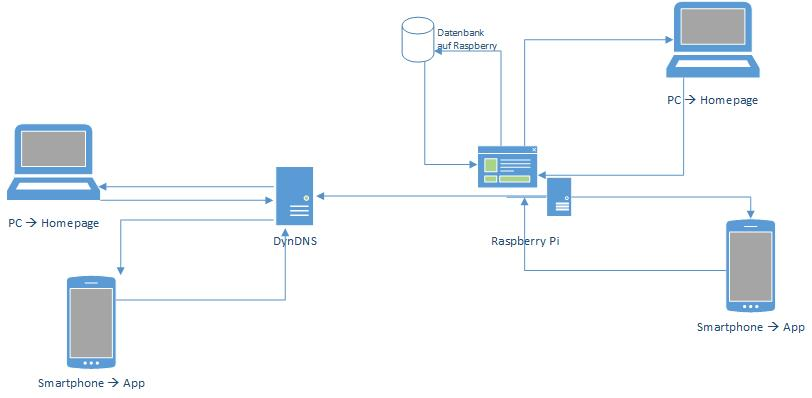
\includegraphics[width=1\textwidth]{netzwerkdiagramm.jpg}
	\caption{Netzwerkdiagramm}
	\label{netzwerkdiagramm}
\end{figure}

\section{Arbeits - Aufteilung}
\subsection{Frau Chüara}
Hauptthema Android App
Die oben aufgezählten Musskriterien für die App sollen von Chiara programmiert und umgesetzt werden.
Die zentrale Datenbank die am Raspberry läuft wird von Chiara angelegt.
\subsection{Herr Filib}
Hauptthema Homepage
Die oben genannten Musskriterien für die Homepage sollen von Philip programmiert und umgesetzt werden.
Die Userverwaltung wird von FLB programmiert.
Die Verwaltung von GitHub wird von Filib verwaltet.

\bigskip 
Die Arbeitsberichte am Ende der Stunde werden von beiden gemeinsam erstellt und upgeloaded.

\end{document}